\section{Introduction}
% problem description: semantic relatedness
Computing semantic relatedness(SR) between two elements(words, sentences,
texts etc.) is a fundamental task for many applications in Natural Language
Processing(NLP) such as lexicon induction\cite{aaai/QadirMGL15}, Named 
Entity Disambiguation\cite{acl/HanZ10}, Keyword Extraction
\cite{ijcai/ZhangFW13} and Information Retrieval\cite{acl/GurevychMZ07}. 
Additionaly, computing semantic relatedness contributes other applications, 
for example, opinion spam problem\cite{www/SandulescuE15}, image classification\cite{iwcs/LeongM11} and so on. 
In this paper we focus on computing semantic relatedness between two 
words in knowledge graph.

It has long been thought that when humans measure the relatedness between
a pair of words, a deeper reasoning is triggered to compare the concepts
behind the words. Many traditional studies on semantic relatedness
utilize different data sources. There are
i) \emph{the large corpora}, such as wikipedia\cite{ijcai/GabrilovichM07},
ii) \emph{the lexical databases}, such as WordNet\cite{acl/Pucher07} or Wikithionary\cite{aaai/ZeschMG08}, 
iii) \emph{the knowledge graph}, such as DBpedia\cite{aaai/NavigliP12} or BabelNet\cite{aaai/NavigliP12}.
With the development of knowledge representation, utilizing knowledge-rich resources to compute semantic 
relatedness is a well-explored line of research. It is known to all that
knowledge graph contains richer syntactic and semantic information than lexical databases,
and more structured knowledge than the large corpora.
On the account of advantages of knowledge graph, we utilize it as background 
knowledge to compute semantic relatedness.

% Knowledge graph can be accessed with powerful query language Sparql in RDF graph.
% As for the methods build on the data soruce, the recent word embedding 
% learning approaches demonstrate their abilities
% to capture syntactic and semantic information, and outperform the
% lexicon-based methods\cite{acl/Pucher07}. 
% Knowledge Graph, as a semantic graph, stores
% vast amount of structured knowledge. 

Recently, there are some researchers having attached importance to measure semantic relatedness
in knowledge graph\cite{acl/IacobacciPN15}, \cite{aaai/NavigliP12}, \cite{aaai/Pirro12}. 
This paper \cite{acl/IacobacciPN15} leveraged entity linking to annotate the dump of wikipedia. Based on this,
the sense-annotated corpus was generated. Then they\cite{acl/IacobacciPN15} used word2vec to
train the sense-annotated corpus and got distributed representation of different 
word senses. This step still needs a significant preprocessing and data transformation efforts. 
As we can see that the author\cite{acl/IacobacciPN15} computed semantic relatedness on account of large corpora.
They just put the knowledge graph on the position of support.
Another paper\cite{aaai/NavigliP12} proposed a knowledge-rich approach to compute multilingual semantic
relatedness which exploited the joint contribution of different languages. Given a pair of words 
in two languages, they\cite{aaai/NavigliP12} utilized BabelNet to collect their translations and computed semantic
relatedness in a variety of languages. Then they combined the empirical evidence from these 
different languages by intersecting their respective graphs.
Another work \cite{aaai/Pirro12} proposed an approach which exploited the graph nature of RDF and SPARQL query
Language to access knowledge graph. It not only obtained the comparable
result with the state-of-art model at that moment, but also avoided the burden
of preprocessing and data transformation.

Though the paper\cite{aaai/Pirro12} avoided a significant preprocessing and data
transformation effort, and develops scalability of their approach while adopting 
the knowledge graph. However, they missed some factors which
might contribute to semantic relatedness measurement. Firstly, given two words
as input, the first step is to find corresponding entities in knowledge
graph. Obviously, there are usually more than one corresponding entities for a single word.
For an input word \emph{car}, for example, we will get \emph{DBPedia:\footnote{http://dbpedia.org/resource}Automobile} and
\emph{DBPedia:Auto\underline{\hspace{0.5em}}Racing} and so on. The work \cite{aaai/Pirro12} losed
sight of the informativeness of the other entities, while they just
consider the entity with the highest rank. Secondly, they \cite{aaai/Pirro12} misseed
some informativeness of \emph{objects} in \emph{triple(subject, prediacte, object)} because their strategy took
the \emph{predicates} into account exclusively based on the TFIDF. This
method ignored the function of \emph{objects} in a semantic triple.

\begin{figure*}
    \centering
    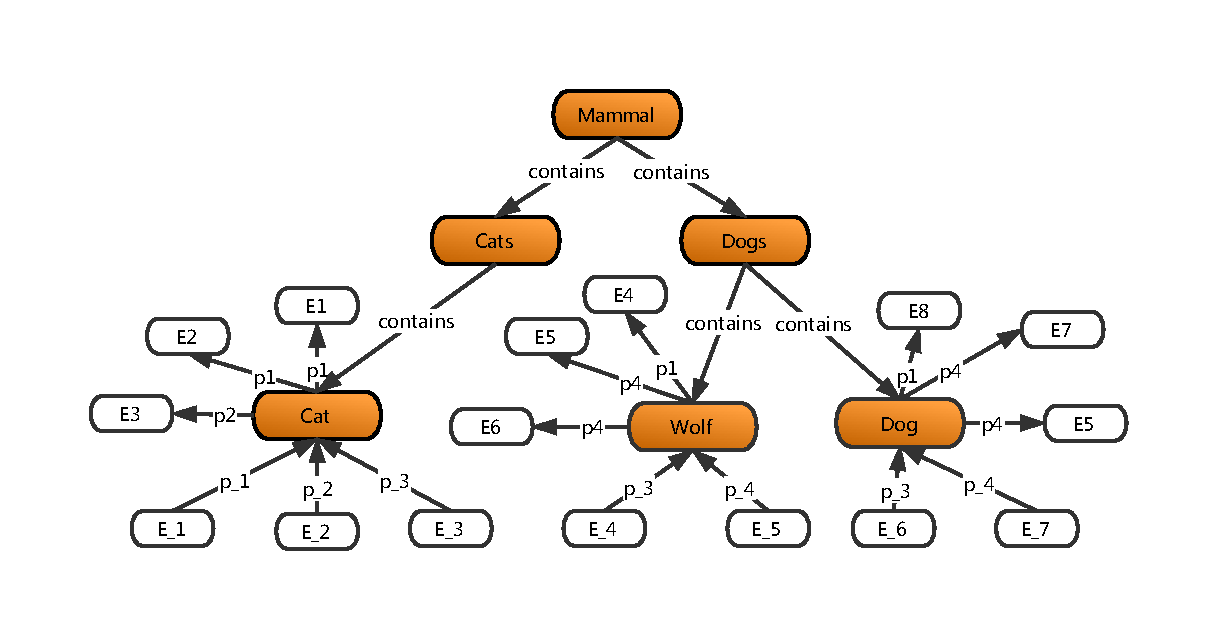
\includegraphics[width=1.1\textwidth]{pic/introduction.pdf}\\
    \caption{Subgraph example in knowledge graph}
    \label{weak1}
\end{figure*}

As show in figure \ref{weak1}, the subgraph contains \emph{Dogs} and \emph{Cats} extracted from
knowledge. We simplify the specific features of \emph{Dogs} and \emph{Cats} to concise symbol shown as $E_i$ in figure. 
We can see that the entity \emph{Cat} plays the role 
of both \emph{Object(Cats contains Cat)} and \emph{Subject(Cat $p_1$ $E_1$)}
in the pattern of triples. The \emph{predicate} which is connected with an entity(Cat)
may be regarded as an outgoing($p_1$) or incoming \emph{predicate}($p_{_1}$).
In the paper\cite{aaai/Pirro12}, the relatedness space for an entity ${E_i}$ is modelled as a 
$k$-dimensional weighted vector \emph{V$_i$}, where each dimension represents
the informativeness of a specific \emph{predicate}.
For example, the weighted vector for \emph{Cat} is 
$[v_{p_1}^o, v_{p_2}^o, v_{p_\_1}^i, v_{p_\_2}^i, v_{p_\_2}^i]$ in which $v_{p_i}^o$ 
means the vector value of outgoing predicate $p_i$ and $v_{p_j}^i$ 
means the vector value of incoming predicate $p_j$.
In this example, from the view of outgoing \emph{predicate} $p_i$, there are three triples
\emph{(Cat $p_1$ $E_1$)}, \emph{(Cat $p_1$ $E_2$)} and \emph{(Cat $p_2$ $E_3$)} which describe the entity \emph{Cat}.
Specifically, in order to compute the vector value of $p_1$,
the way of paper \cite{aaai/Pirro12} in which they got the informativeness of $p_i$ was to count the number
of triples with the form of \emph{(Cat $p_1$ ?)} firstly, then they divided this result
by the total number of triples in which \emph{Cat} appears
((Cat $p_1$ $E_1$), (Cat $p_1$ $E_2$), (Cat $p_2$ $E_3$)), i.e., $v_{p_1}^o$=2/3.
They\cite{aaai/Pirro12} only considered the informativeness of \emph{prediacte},
and ignored the function of a set of specific \emph{objects} in a pattern of triple.
Besides, there is another aspect they have ignored. In this example, for entities $Cat$,
$Dog$ and $Wolf$, let us see the informativeness of prediacte $p_1$. We get
\emph{(Cat $p_1$ $E_1$), (Cat $p_1$ $E_2$), (Wolf $p_1$ $E_4$)} and \emph{(Dog $p_1$ $E_8$)}. 
It is obvious that when they\cite{aaai/Pirro12} computed relatedness between \emph{Cat} and \emph{Wolf}, 
they got the same vector value for predicate $p_1$ both in the aspect of \emph{Wolf} and \emph{Dog}.
In other words, in the dimension of predicate $p_1$ vector between pair (\emph{Cat},\emph{Wolf}) and
(\emph{Cat},\emph{Dog}), they got no difference. Accordingly, they did not distinguish the different
objects for a specific predicate. In order to improve the performance of 
semantic relatedness measurement based on knowledge graph, we propose a threefold model which is shown as follows:

1. For given a pair of words, the first job is to query the corresponding entities. In order to use the
neural network for training the dataset, we also need to construct a graph which contains all related
entities, attributes and relations between the corresponding entity pairs.

2. We use Starspace proposed by Facebook for knowledge graph instead of Word2vec to train the subgraph
extracted from the knowledge graph. Then we can get a distributional representation(vector) for each
entity and predicate. 

3. When we take as inputs a pair of words, we can get two sets of corresponding entities queried from
knowledge graph. Then we can get multiple relatedness scores after a full link between these two sets of entities.
Inspired by \cite{acl/IacobacciPN15}, we utilize an approach to combine the 
relatedness scores as the final semantic relatedness score in knowledge graph.

This paper is organized as follows. We give the related work about semantic relatedness
measurement in section \ref{related-word}. Then we elaborate the threefold model for
computing relatedness scores in section \ref{methodlogy}. Finally, we display detailed
illustrations of experiment results which show that our model outperform the state-of-the-art model.